% This is the template used for the GIH thesis. It is based on 
% Reed College LaTeX thesis template. Most of the work (Reed template)
% for the document class was done by Sam Noble (SN), as well as this
% template. Later comments etc. by Ben Salzberg (BTS). Additional
% restructuring and APA support by Jess Youngberg (JY).
%
% See http://web.reed.edu/cis/help/latex.html for help. There are a
% great bunch of help pages there, with notes on
% getting started, bibtex, etc. Go there and read it if you're not
% already familiar with LaTeX.
%
% Any line that starts with a percent symbol is a comment.
% They won't show up in the document, and are useful for notes
% to yourself and explaining commands.
% Commenting also removes a line from the document;
% very handy for troubleshooting problems. -BTS

% The template was updated by Daniel Hammarström to fit GIH
% requirements. Additional code was borrowed from the 
% Stockholm University (Andreas Solders 2011) template.

% The template was forked from the thesisdown package (CII updates)

%%
%% Preamble
%%
% \documentclass{<something>} must begin each LaTeX document
\documentclass[twoside,10pt]{gihclass} %Default style using S5 paper
% Packages are extensions to the basic LaTeX functions. Whatever you
% want to typeset, there is probably a package out there for it.
% Chemistry (chemtex), screenplays, you name it.
% Check out CTAN to see: http://www.ctan.org/
%%
\usepackage{graphicx,latexsym}
\usepackage{amsmath}
\usepackage{amssymb,amsthm}
\usepackage{longtable,booktabs,setspace}
\usepackage{chemarr} %% Useful for one reaction arrow, useless if you're not a chem major
\usepackage[hyphens]{url}
% Added by CII
\usepackage{hyperref,xcolor}
\hypersetup{
    colorlinks = false,
    pdfborder={0 0 0}
}
\usepackage{lmodern}
\usepackage{float}
\floatplacement{figure}{H}
% End of CII addition
\usepackage{rotating}

% Next line commented out by CII
%%% \usepackage{natbib}
% Comment out the natbib line above and uncomment the following two lines to use the new
% biblatex-chicago style, for Chicago A. Also make some changes at the end where the
% bibliography is included.
%\usepackage{biblatex-chicago}
%\bibliography{thesis}


% Added by CII (Thanks, Hadley!)
% Use ref for internal links
\renewcommand{\hyperref}[2][???]{\autoref{#1}}
\def\chapterautorefname{Chapter}
\def\sectionautorefname{Section}
\def\subsectionautorefname{Subsection}
% End of CII addition

% Added by CII
\usepackage{caption}
\captionsetup{width=5in}
% End of CII addition


% \usepackage{times} % other fonts are available like times, bookman, charter, palatino

% Syntax highlighting #22

% To pass between YAML and LaTeX the dollar signs are added by CII

% New variables 2019-02-06 GIH copyright info 
\isbn{Provided by the library} 
\place{Stockholm}
\printeby{Printer service, Stockholm, 2019}
\coverinfo{}
\year{2019}



\title{Determinants of intra-individual variation in adaptability to resistance training of different volumes with special reference to skeletal muscle phenotypes}
\author{Daniel Hammarström}
% The month and year that you submit your FINAL draft TO THE LIBRARY (May or December)
\date{May 20xx}


%If you have two advisors for some reason, you can use the following
% Uncommented out by CII
\sernr{999}
% End of CII addition
%%% Remember to use the correct department!

% if you're writing a thesis in an interdisciplinary major,
% uncomment the line below and change the text as appropriate.
% check the Senior Handbook if unsure.
%\thedivisionof{The Established Interdisciplinary Committee for}
% if you want the approval page to say "Approved for the Committee",
% uncomment the next line
%\approvedforthe{Committee}

% Added by CII
%%% Copied from knitr
%% maxwidth is the original width if it's less than linewidth
%% otherwise use linewidth (to make sure the graphics do not exceed the margin)
\makeatletter
\def\maxwidth{ %
  \ifdim\Gin@nat@width>\linewidth
    \linewidth
  \else
    \Gin@nat@width
  \fi
}
\makeatother

\renewcommand{\contentsname}{Table of Contents}
% End of CII addition

\setlength{\parskip}{0pt}

% Added by CII

\providecommand{\tightlist}{%
  \setlength{\itemsep}{0pt}\setlength{\parskip}{0pt}}




\Dedication{
You can have a dedication here if you wish.
}

\Preface{

}

\Abstract{
The preface pretty much says it all.

\par

Second paragraph of abstract starts here.
}

	\usepackage[utf8]{inputenc}
\usepackage[T1]{fontenc}
\usepackage{libertine}
\usepackage{lettrine}
\usepackage[svgnames]{xcolor}
% End of CII addition
%%
%% End Preamble
%%
%
\begin{document}




% Everything below added by CII


\frontmatter % this stuff will be roman-numbered
% \pagestyle{empty} % this removes page numbers from the frontmatter
  \maketitle
  \begin{dedication}
  \topskip0pt
\vspace*{\fill}
 You can have a dedication here if you wish.
\vspace*{\fill}
  \end{dedication}
\begin{defence}
    THESIS FOR DOCTORAL DEGREE (Ph.D.)\\
    ~\\
    ~\\
    \textbf{The title of your thesis}\\
    ~\\
    by\\
    \textbf{Your name}\\
    ~\\
    ~\\
    Thesis for Philosophy of Doctoral Degree in Sport Sciences, at The Swedish School of Sport and Health Sciences (GIH), which, according to the decision of the dean, will be publicly defended on \emph{DATE}. The thesis defense will be held at the auditorium at The Swedish School of Sport and Health Sciences (GIH), Stockholm.\\
    ~\\
    ~\\
    \textbf{Opponent}\\
    Profesor \ldots.\\
    ~\\
    \textbf{Principal supervisor}\\
    Profesor\ldots{}\\
    ~\\
    \textbf{Co-supervisor(s)}\\
    -Professor\ldots{}\\
    -Professor\ldots{}\\
    -Professor\ldots{}\\
    ~\\
    \textbf{Examination board}\\
    -Associate professor\ldots{}\\
    -Professor \ldots{}\\
    -Professor \ldots{}
  \end{defence}

  \begin{abstract}
    The preface pretty much says it all.
    
    \par
    
    Second paragraph of abstract starts here.
  \end{abstract}



  \hypersetup{linkcolor=black}
  \setcounter{tocdepth}{2}
  \tableofcontents

  \listoftables

  \listoffigures




\mainmatter % here the regular arabic numbering starts
\pagestyle{fancyplain} % turns page numbering back on

\setcounter{DefaultLines}{3}

\hypertarget{introduction}{%
\chapter{Introduction}\label{introduction}}

\lettrine[findent=3pt, nindent=0pt, ante=\rlap{\color{LightSalmon!50}\rule[-0.55\LettrineHeight]{\LettrineWidth}{0.65\LettrineHeight}} ]{P}\{roper\} former days -- that is to say, once upon a time, there lived in the Land of Gramblamble, Seven Families. They lived by the side of the great Lake Pipple-popple (one of the Seven Families, indeed, lived in the Lake), and on the outskirts of the City of Tosh, which, excepting when it was quite dark, they could see plainly. The names of all these places you have probably heard of, and you have only not to look in your Geography books to find out all about them.
skeletal muscle functioning is essential in everyday life by enabling movement and thus complex interaction with our environment. Nutrition and pharmacological agents can have substantial effects on skeletal muscle mass and function. However, resistance exercise of sufficient volume, intensity and frequency is the most potent stimuli to promote morphological and functional changes in the human neuromuscular system. Exercise training can be modulated indefinitely by combining different variations of training variables and in addition, adaptation to exercise training is a phenomenon characterized by great inter-individual variability. The purpose of the present project is therefore to explore potential determinants of variation in adaptability to resistance-exercise modulated by selected exercise-training variables.

(Pinedo-Villanueva et al., 2019)

\hypertarget{background}{%
\chapter{Background}\label{background}}

\hypertarget{exercise-training-variables-affecting-training-outcomes}{%
\section{Exercise training variables affecting training outcomes}\label{exercise-training-variables-affecting-training-outcomes}}

\hypertarget{exercise-volume}{%
\section{Exercise volume}\label{exercise-volume}}

\hypertarget{meta-analysis-of-exercise-volume}{%
\subsection{Meta-analysis of exercise volume}\label{meta-analysis-of-exercise-volume}}

\hypertarget{molecular-determinants-of-training-induced-muscle-hypertrophy}{%
\section{Molecular determinants of training-induced muscle hypertrophy}\label{molecular-determinants-of-training-induced-muscle-hypertrophy}}

\hypertarget{protein-synthesis}{%
\subsection{Protein synthesis}\label{protein-synthesis}}
\begin{figure}
\centering
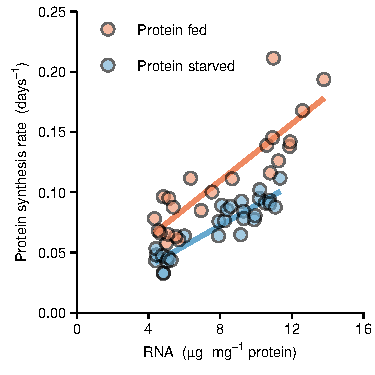
\includegraphics{thesis_files/figure-latex/Millward1973-1.pdf}
\caption{\label{fig:Millward1973}Data from Millward et al.~1973. Group A were fed a diet containing protein, group B were starved or fed a diet not containing protein.}
\end{figure}
\hypertarget{the-mammalian-target-of-rapamycin-mtor-and-translational-efficiency}{%
\subsection{The mammalian target of rapamycin (mTOR) and translational efficiency}\label{the-mammalian-target-of-rapamycin-mtor-and-translational-efficiency}}

The mammalian target of rapamycin (mTOR) is a large serine-threonine protein kinase wich in complex with oyher regulatory proteins forms a signaling hub responsible for responses to environmental cues such as nutrients and mechanical stress.

mTOR has several phosphorylation sites

Phosphorylation of Ser2448 is mediated by S6K1 to reduce mTOR activity in a negative feedback loop .

Ser2448 is phosphorylated by S6K1, changes in nutrient avaliability modifies S6K1 and Ser2448, Ser2448 phosphorylation is abolished when S6K1 is depleted

When the C-terminal is deleted, mTOR gets constitutively active

\hypertarget{ribsome-biogenesis}{%
\subsection{Ribsome biogenesis}\label{ribsome-biogenesis}}

\hypertarget{transcription-of-ribsomal-rna-rrna}{%
\subsubsection{Transcription of ribsomal RNA (rRNA)}\label{transcription-of-ribsomal-rna-rrna}}

\hypertarget{transcriptional-activity-related-to-muscle-hypertrophy}{%
\section{Transcriptional activity related to muscle hypertrophy}\label{transcriptional-activity-related-to-muscle-hypertrophy}}

\hypertarget{methods-for-studying-transcriptional-regulation}{%
\subsection{Methods for studying transcriptional regulation}\label{methods-for-studying-transcriptional-regulation}}

\hypertarget{aims-and-hypotheses}{%
\chapter{Aims and hypotheses}\label{aims-and-hypotheses}}

\hypertarget{methods}{%
\chapter{Methods}\label{methods}}

TO DO:
\begin{itemize}
\tightlist
\item
  For methods discussion, compare product length, efficiencies and ct values in relation to RQI-values. See Fleige 2006 for reference.
\end{itemize}
\hypertarget{training-protocols}{%
\section{Training protocols}\label{training-protocols}}

A full body protocol was used in study I including

\hypertarget{results}{%
\chapter{Results}\label{results}}

\hypertarget{discussion}{%
\chapter{Discussion}\label{discussion}}

\hypertarget{conclusion}{%
\chapter*{Conclusion}\label{conclusion}}
\addcontentsline{toc}{chapter}{Conclusion}

If we don't want Conclusion to have a chapter number next to it, we can add the \texttt{\{-\}} attribute.

\textbf{More info}

And here's some other random info: the first paragraph after a chapter title or section head \emph{shouldn't be} indented, because indents are to tell the reader that you're starting a new paragraph. Since that's obvious after a chapter or section title, proper typesetting doesn't add an indent there.

\backmatter

\hypertarget{references}{%
\chapter*{References}\label{references}}
\addcontentsline{toc}{chapter}{References}

\markboth{References}{References}

\noindent

\setlength{\parindent}{-0.20in}
\setlength{\leftskip}{0.20in}
\setlength{\parskip}{8pt}

\hypertarget{refs}{}
\leavevmode\hypertarget{ref-RN2184}{}%
Pinedo-Villanueva, R., Westbury, L. D., Syddall, H. E., Sanchez-Santos, M. T., Dennison, E. M., Robinson, S. M., \& Cooper, C. (2019). Health care costs associated with muscle weakness: A uk population-based estimate. \emph{Calcif Tissue Int}, \emph{104}(2), 137--144. Journal Article. \url{http://doi.org/10.1007/s00223-018-0478-1}


% Index?

\end{document}
